\section{Data sources}
\subsection{YouTube}
\subsubsection{YouTube data}
YouTube stores various data concerning its users and content. Tables
\ref{ut_video_info} - \ref{ut_channel_info} show the types of information
available.

\begin{table}[ht]
	\begin{tabular}{|p{3cm} | l | p{4cm}|}\hline
		Information & Access & Description\\ \hline

		Title & Public API & \\
		Published & Public API & \\
		Updated & Public API & \\
		Category & Public API & \\
		Tags (keywords) & Public API & \\
		Comments & Public API & \\
		Permissons & Public API & \\
		Description & Public API & \\
		Thumbnails & Public API & Set of video's thumbnails (along with times
		when taken) \\
		Duration & Public API & \\
		Ratings & Public API & Best, worst and average rating, number of votes \\
		Viewcount & Public API & \\
		Favourite count & Public API & \\
		Number of likes & Public API & \\
		Number of dislikes & Public API & \\
		Aspect ratio & Public API & \\
		Related & Public API & \\
		Responses & Public API & \\
		Author & Public API & \\ \hline
	\end{tabular}
	\caption{Information available for a video}
\end{table}

\begin{table}[ht]
	\begin{minipage}[b]{0.5\linewidth}
	\centering
		\begin{tabular}{ | p{3cm} | l |}\hline
		Information & Access \\ \hline
		Number of results & Public API \\
		Search results & Public API \\ \hline
		\end{tabular}
		\caption{Information available for video search results}
	\end{minipage}
	\hspace{0.5cm} % no new lines here!!
	\begin{minipage}[b]{0.5\linewidth}
		\centering
		\begin{tabular}{ | p{3cm} | l |}\hline
			Information & Access\\ \hline
			Uploads & Public API \\
			Gender & Public API \\
			Location & Public API \\
			Age & Public API \\
			Contacts & Public API \\
			Username & Public API \\
			Subscriptions & Public API \\
			Inbox & Public API \\
			Favorites & Public API \\
			History & Screen scraping \\
			Likes & Screen scraping \\
			Issued authentication subtokens & Screen scraping \\ \hline
		\end{tabular}
		\caption{Information available for a user}
	\end{minipage}
\end{table}


\begin{table}[ht]
	\begin{minipage}[b]{0.5\linewidth}\centering
		\begin{tabular}{ | p{3cm} | l |}\hline
			Information & Access \\ \hline
			Created & Public API \\
			Updated & Public API \\
			Author & Public API \\
			Text & Public API \\ \hline
		\end{tabular}
		\caption{Information available for a comment}
	\end{minipage}
	\hspace{0.5cm} % no new lines here!!
	\begin{minipage}[b]{0.5\linewidth}
		\centering
		\begin{tabular}{ | p{3cm} | l |}\hline
			Information & Access \\ \hline
			Demographics & Screen scraping \\
			Referrers & Screen scraping \\
			Countries popularity & Screen scraping \\ \hline
		\end{tabular}
		\caption{Information available for a channel}
	\end{minipage}
\end{table}


\subsubsection{YouTube usage}

A statistics were performed measuring popularity of three YouTube features: favourites,
subscriptions and uploads. Over a sample of 7500 users most settled down at
relatively low level of activity. All histograms below show numbers of users
(axis y) with $x_1-x_2$ numbers of favourites/subscriptions/uploads. The
logarithmic scale was used for all three charts.

\begin{figure}[ht]
  \centering
  \subfigure[Favourites]{
		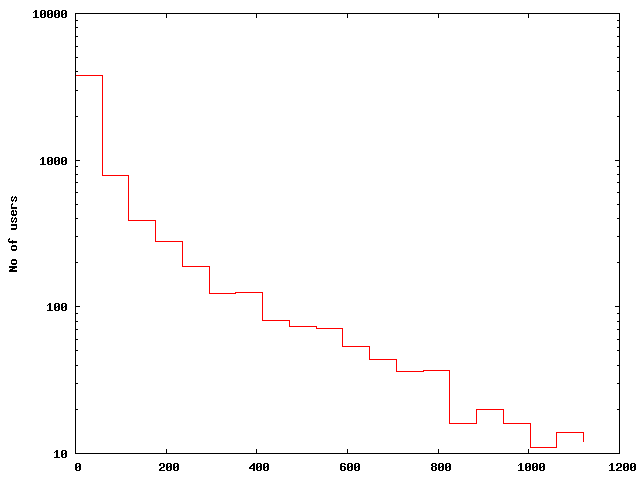
\includegraphics[scale=0.6]{images/favs.png}
		\label{fig:favs}
  }
  \subfigure[Subscriptions]{
		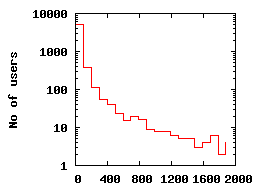
\includegraphics[scale=0.6]{images/subs.png}
		\label{fig:subs}
  }
  \subfigure[Uploads]{
		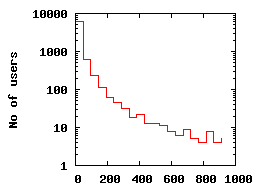
\includegraphics[scale=0.6]{images/ups.png}
		\label{fig:ups}
  }
  \label{fig:subfigureExample}
  \caption{Histograms of usage of favourites \subref{fig:favs}, subscriptions
  \subref{fig:subs} and uploads \subref{fig:ups}. The x axis represents groups of
  users having $x_1-x_2$ entities, the height of the bars indicates sizes of the
  groups.}
\end{figure}

